\documentclass[a4paper,12pt]{book}
% Paquetes de la ams
\usepackage{amsmath,amsthm,amssymb,amsfonts}
% Codificacion UTF-8
\usepackage[utf8]{inputenc}
% Tablas e imagenes en espaniol
\usepackage[spanish,es-tabla]{babel}
% Mejores graficos
\usepackage{graphicx}
% tablas mas lindas
\usepackage{booktabs}
% Links a urls
\usepackage{url}
% Linkear referencias en pdfs
\usepackage{hyperref}
% Texto mas lindo para los pie de figura
\usepackage[margin=10pt,font=small,labelfont=bf, labelsep=endash]{caption}

% Citas
\usepackage[backend=biber,style=ieee]{biblatex}
\addbibresource{biblio.bib}

% Codigo
\usepackage{listings}

% Dir tree
\usepackage{dirtree}

% Pagina en blanco cuando ha
\usepackage{emptypage}

\definecolor{A11}{HTML}{B2DF8A}
\definecolor{A12}{HTML}{33A02C}
\definecolor{A23}{HTML}{FDBF6F}
\definecolor{A24}{HTML}{FF7F00}
\definecolor{B15}{HTML}{FB9A99}
\definecolor{B16}{HTML}{E31A1C}
\definecolor{B27}{HTML}{A6CEE3}
\definecolor{B28}{HTML}{1F78B4}

% Ejemplos, observaciones y teorema
\theoremstyle{definition}
\newtheorem{exa}{Ejemplo}[section]
\newtheorem*{obs}{Observación}
\newtheorem{que}{Pregunta}[section]
\newtheorem{dex}{Definicion}[section]

\usepackage{float}
\graphicspath{{./figs/}}

\title{{\large Nivel 0} \\ Interpretación visual de imágenes satelitales}
\author{Marina Compagnucci \and Francisco Nemiña}
\begin{document}
\maketitle
\titlepage

\chapter{Introducción}
Existen en la actualidad distintas formas de acceder a productos de origen satelital. Es posible obtener resultados que varían desde imágenes en crudo hasta mapas de propiedades y usos del suelo.

En los últimos años, además de las formas tradicionales de procesamiento de imágenes, donde un usuario debía descargar un producto y luego manipularlo, comenzaron a aparecer soluciones web, permitiendo el acceso a un amplio abanico de productos, independientemente de su nivel de conocimiento. Entre ellas se destacan el \href{https://explorer.earthengine.google.com/#workspace}{EarthEngine} de Google, el \href{http://landsatexplorer.esri.com/}{LandsatExplorer} de ESRI, el \href{http://apps.sentinel-hub.com/eo-browser/}{EO Browser} de Sentinel-hub y el \href{lv.eosda.com}{Land Viewer} de EOS.
%ver
No obstante esta posibilidad, es importante disponer de capacitaciones que permitan mejorar el uso de las herramientas. Este taller pretende incorporar los conocimientos básicos de teledetección óptica en interpretación visual, para que los usuarios sin conocimientos previos, puedan acercarce al manejo de productos satelitales de forma clara y sencilla.
%ver
Se trabajará con la aplicación Land Viewer, con el objetivo de analizar los efectos producidos por el invendio en las cercanias de Carlos Paz, provincia de Córdoba en septiembre de 2017.

\chapter{Land Viewer}

LandView es un servicio web de la empresa Earth Observing System, el cual permite explorar, visualizar y descargar, de forma gratuita, hasta 10 imagenes por día de sensores que incluyen la serie \href{https://landsat.usgs.gov/}{Landsat} (1982-actualidad), \href{https://lpdaac.usgs.gov/dataset_discovery/modis/modis_products_table/mcd43a4}{MODIS} (2013-actualidad) y \href{https://sentinel.esa.int/web/sentinel/missions/sentinel-2}{Sentinel 2} (2012-actualidad). % yo no pondría o que esta entre parentesis.

\section{Registro}
Para acceder al servicio de LandView debe dirigirse a \url{https://lv.eosda.com} y registrarse

\section{Interface gráfica}

Una vez que ingresa, accederá a un mapa  similar al de Google Maps (Figura \ref{fig:main}). % pondria una única figura
Destacamos en el tres partes:

\begin{figure}[hb!]
    \centering
    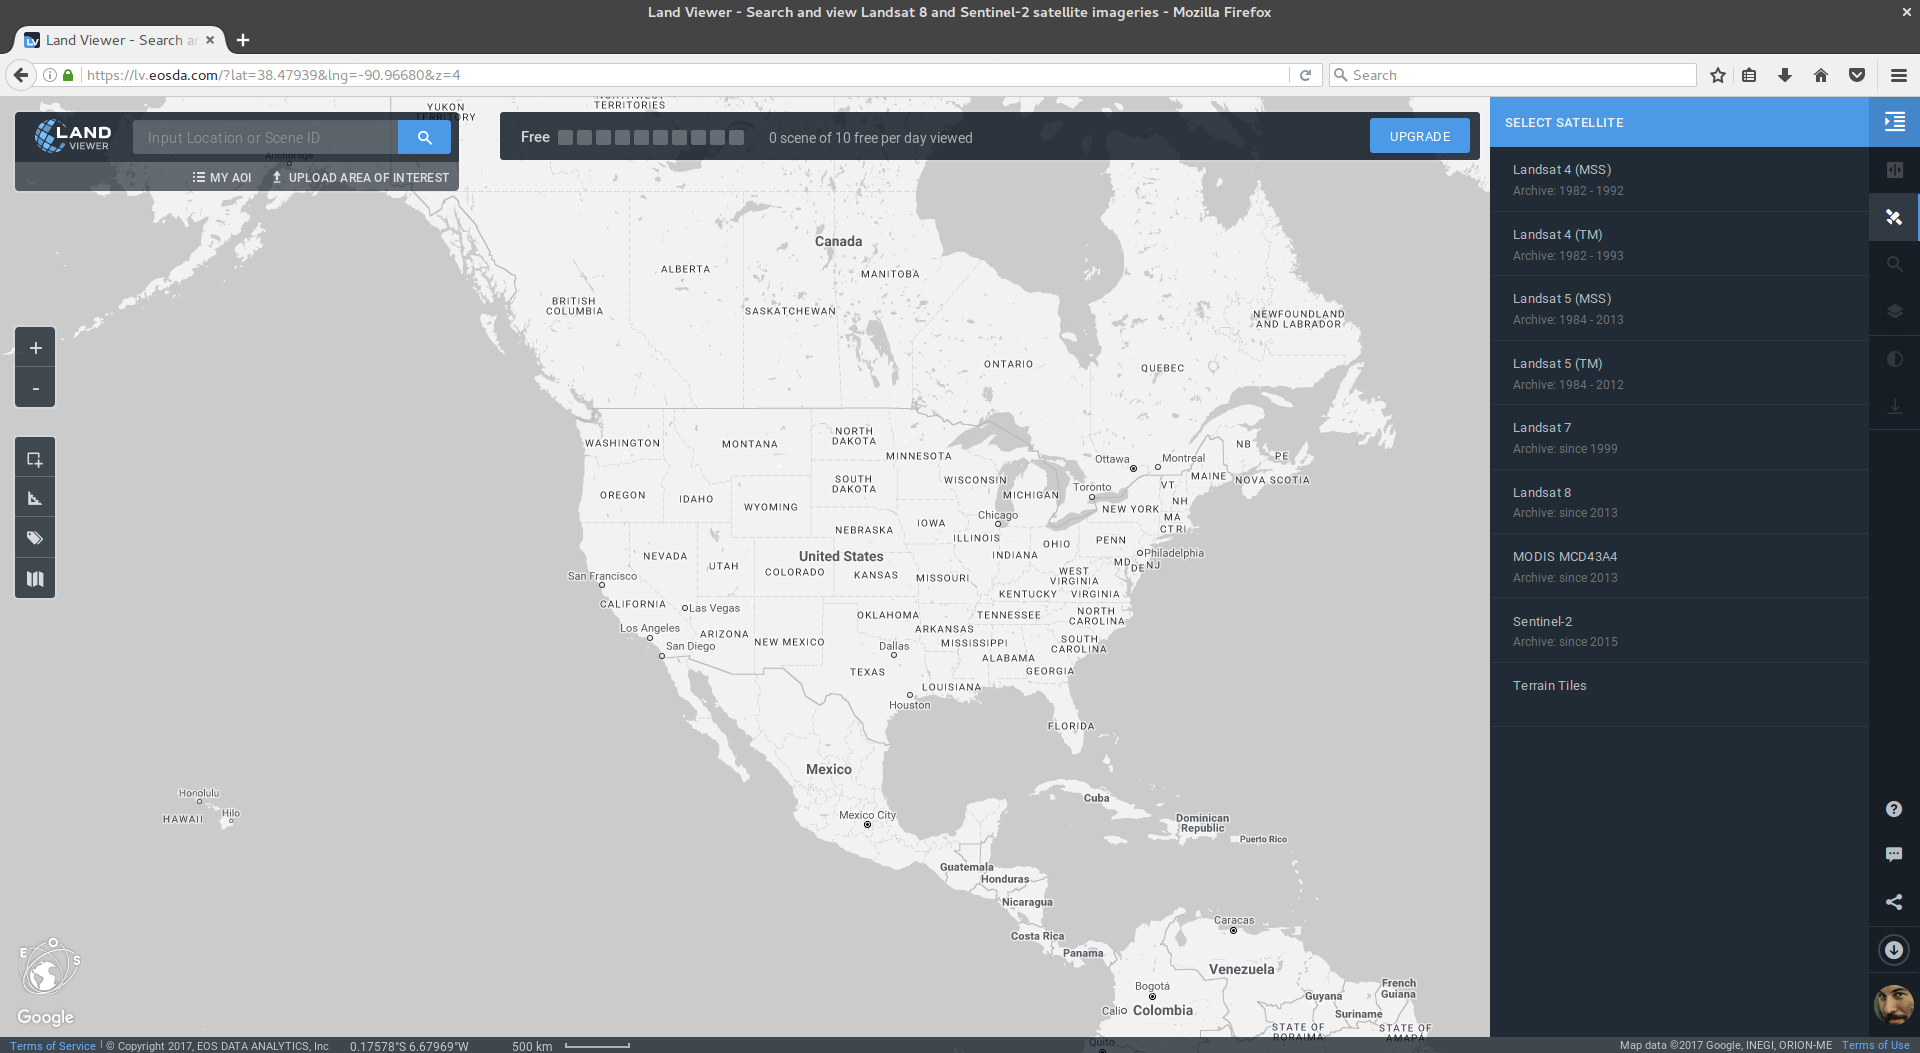
\includegraphics[width=0.85\textwidth]{fig:main.png}
    \caption{Pantalla principal del Land Viewer. Abajo a derecha de encuentra la opción de registro. A la derecha tenemos las herramietas de medición, zoom y mapas. Arriba el cuadro de busqueda. A la izquierda encontramos la selección de imágenes y productos satelitales.}
    \label{fig:main}
\end{figure}

\begin{itemize}
    \item La parte superior que nos permite buscar en el mundo.
     \begin{center}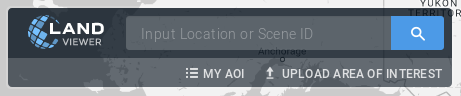
\includegraphics[scale=0.4]{in:search.png}\end{center}
    \item La parte izquierda que nos permite hacer zoom en el mapa, marcar zonas de interés, realizar mediciones y agregar distintas capas como puede ser un mapa de alturas, una imagen satelital de base o un mapa político.
     \begin{center}
\includegraphics[scale=0.4]{in:edit.png}\end{center}
    \item La parte derecha donde podemos elegir distintos productos satelitales, mostrarlos, realizar combinaciones de bandas y guardar los datos obtenidos.
     \begin{center}
\includegraphics[scale=0.4]{in:sat.png}\end{center}
\end{itemize}

Podemos ver tambien la latitud y longitud de cualquier punto posicionandonos sobre el y observando el valor en la parte inferior de la pantalla.




\section{Mediciones}

En el mapa, busque la ciudad de Villa Carlos Paz. Podrá ver sus coordenadas en el margen inferior izquierdo. Utilice la herramienta "Medir distancias" 
\includegraphics[scale=0.2]{in:medir.png} la distancia entre Córdoba Capital y Villa Carlos Paz (Figura \ref{fig:distancia}). Para realizaro, haga un click en el sitiode inicio y otro en el lugar de finalización.

\begin{figure}[!h]
    \centering
    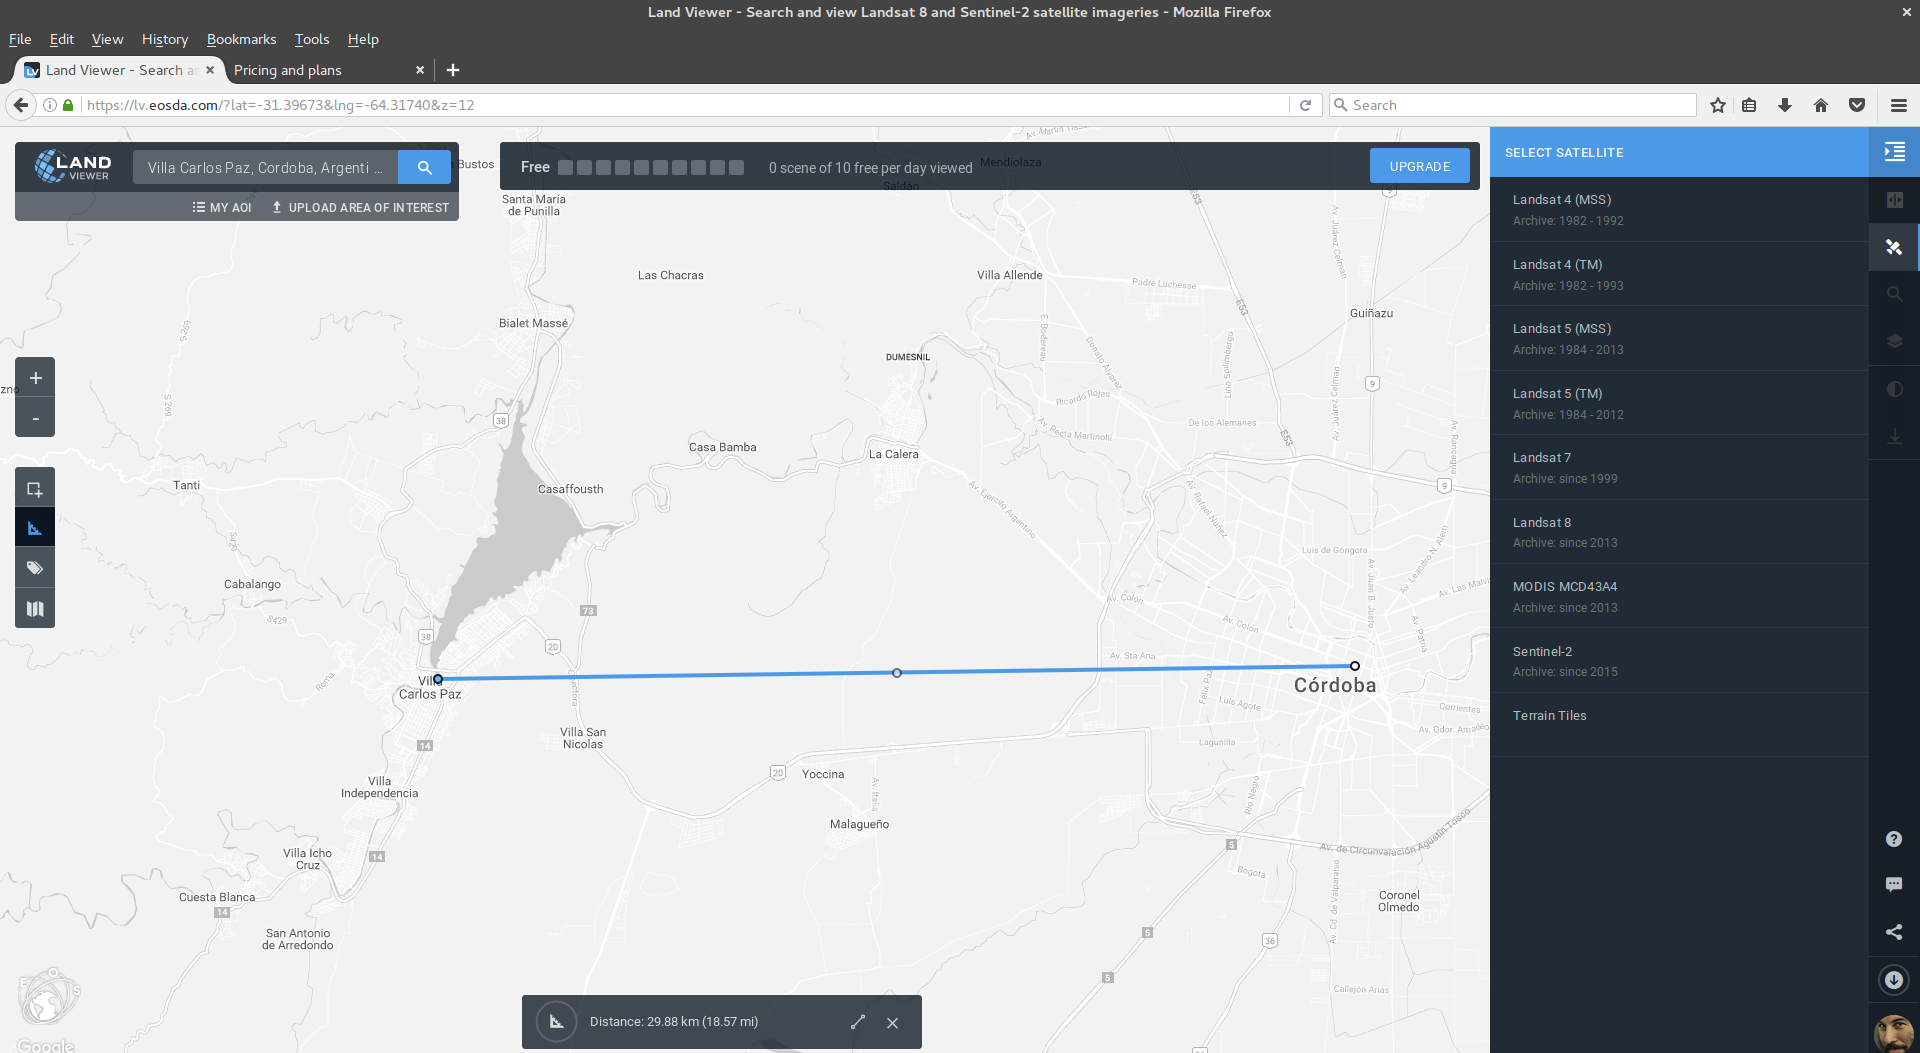
\includegraphics[width=0.85\textwidth]{fig:distancia.png}
    \caption{Medición de distancia entre la ciudad de Córdoba y Villa Carlos Paz. El valor aparece en la parte inferior de la pantalla.}
    \label{fig:distancia}
\end{figure}

Puede medir un área cerrando el polígono sobre el punto inicial.

\section{Actividades}

\begin{que}
    ¿Cuál es la superficie del Lago San Roque, que se encuentra al norte de Villa Carlos Paz?
\end{que}
\begin{que}
    ¿Cuál es el perímetro del Lago San Roque?
\end{que}
\begin{que}
    ¿Cuál es la superficie de la Laguna Mar Chiquita que se encuentra en Córdoba?
\end{que}

\begin{que}
    ¿Cuál es la distancia lineal entre la ciudad de Córdoba y la ciudad de Santa Rosa, La Pampa?
\end{que}

\begin{que}
    ¿Cuales son las coordenadas de las ciudades de Córdoba Capital, Villa Carlos Paz, Rio Cuarto y Villa Maria?
\end{que}




\chapter{Resolución espacial y temporal}
Dos características fundamenteles de las imágenes satelitales son la resolución espacial y la resolución temporal. La primera da una idea de que objetos podemos distinguir en el terreno. Por ejemplo, una resolución espacial de $30m$ nos permitirá distinguir una plaza de una manzana construida, pero no las casas dentro de una manzana.

La resolución temporal indica la la duración del fenomeno ma chico que se puede detectar. Por ejemplo, una resolución temporal de $15$ días posibilita estudiar como cambia la vegetación a lo largo de las estaciones, pero no la variación de nubes a lo largo del día.

\begin{figure}[h!]
    \centering
    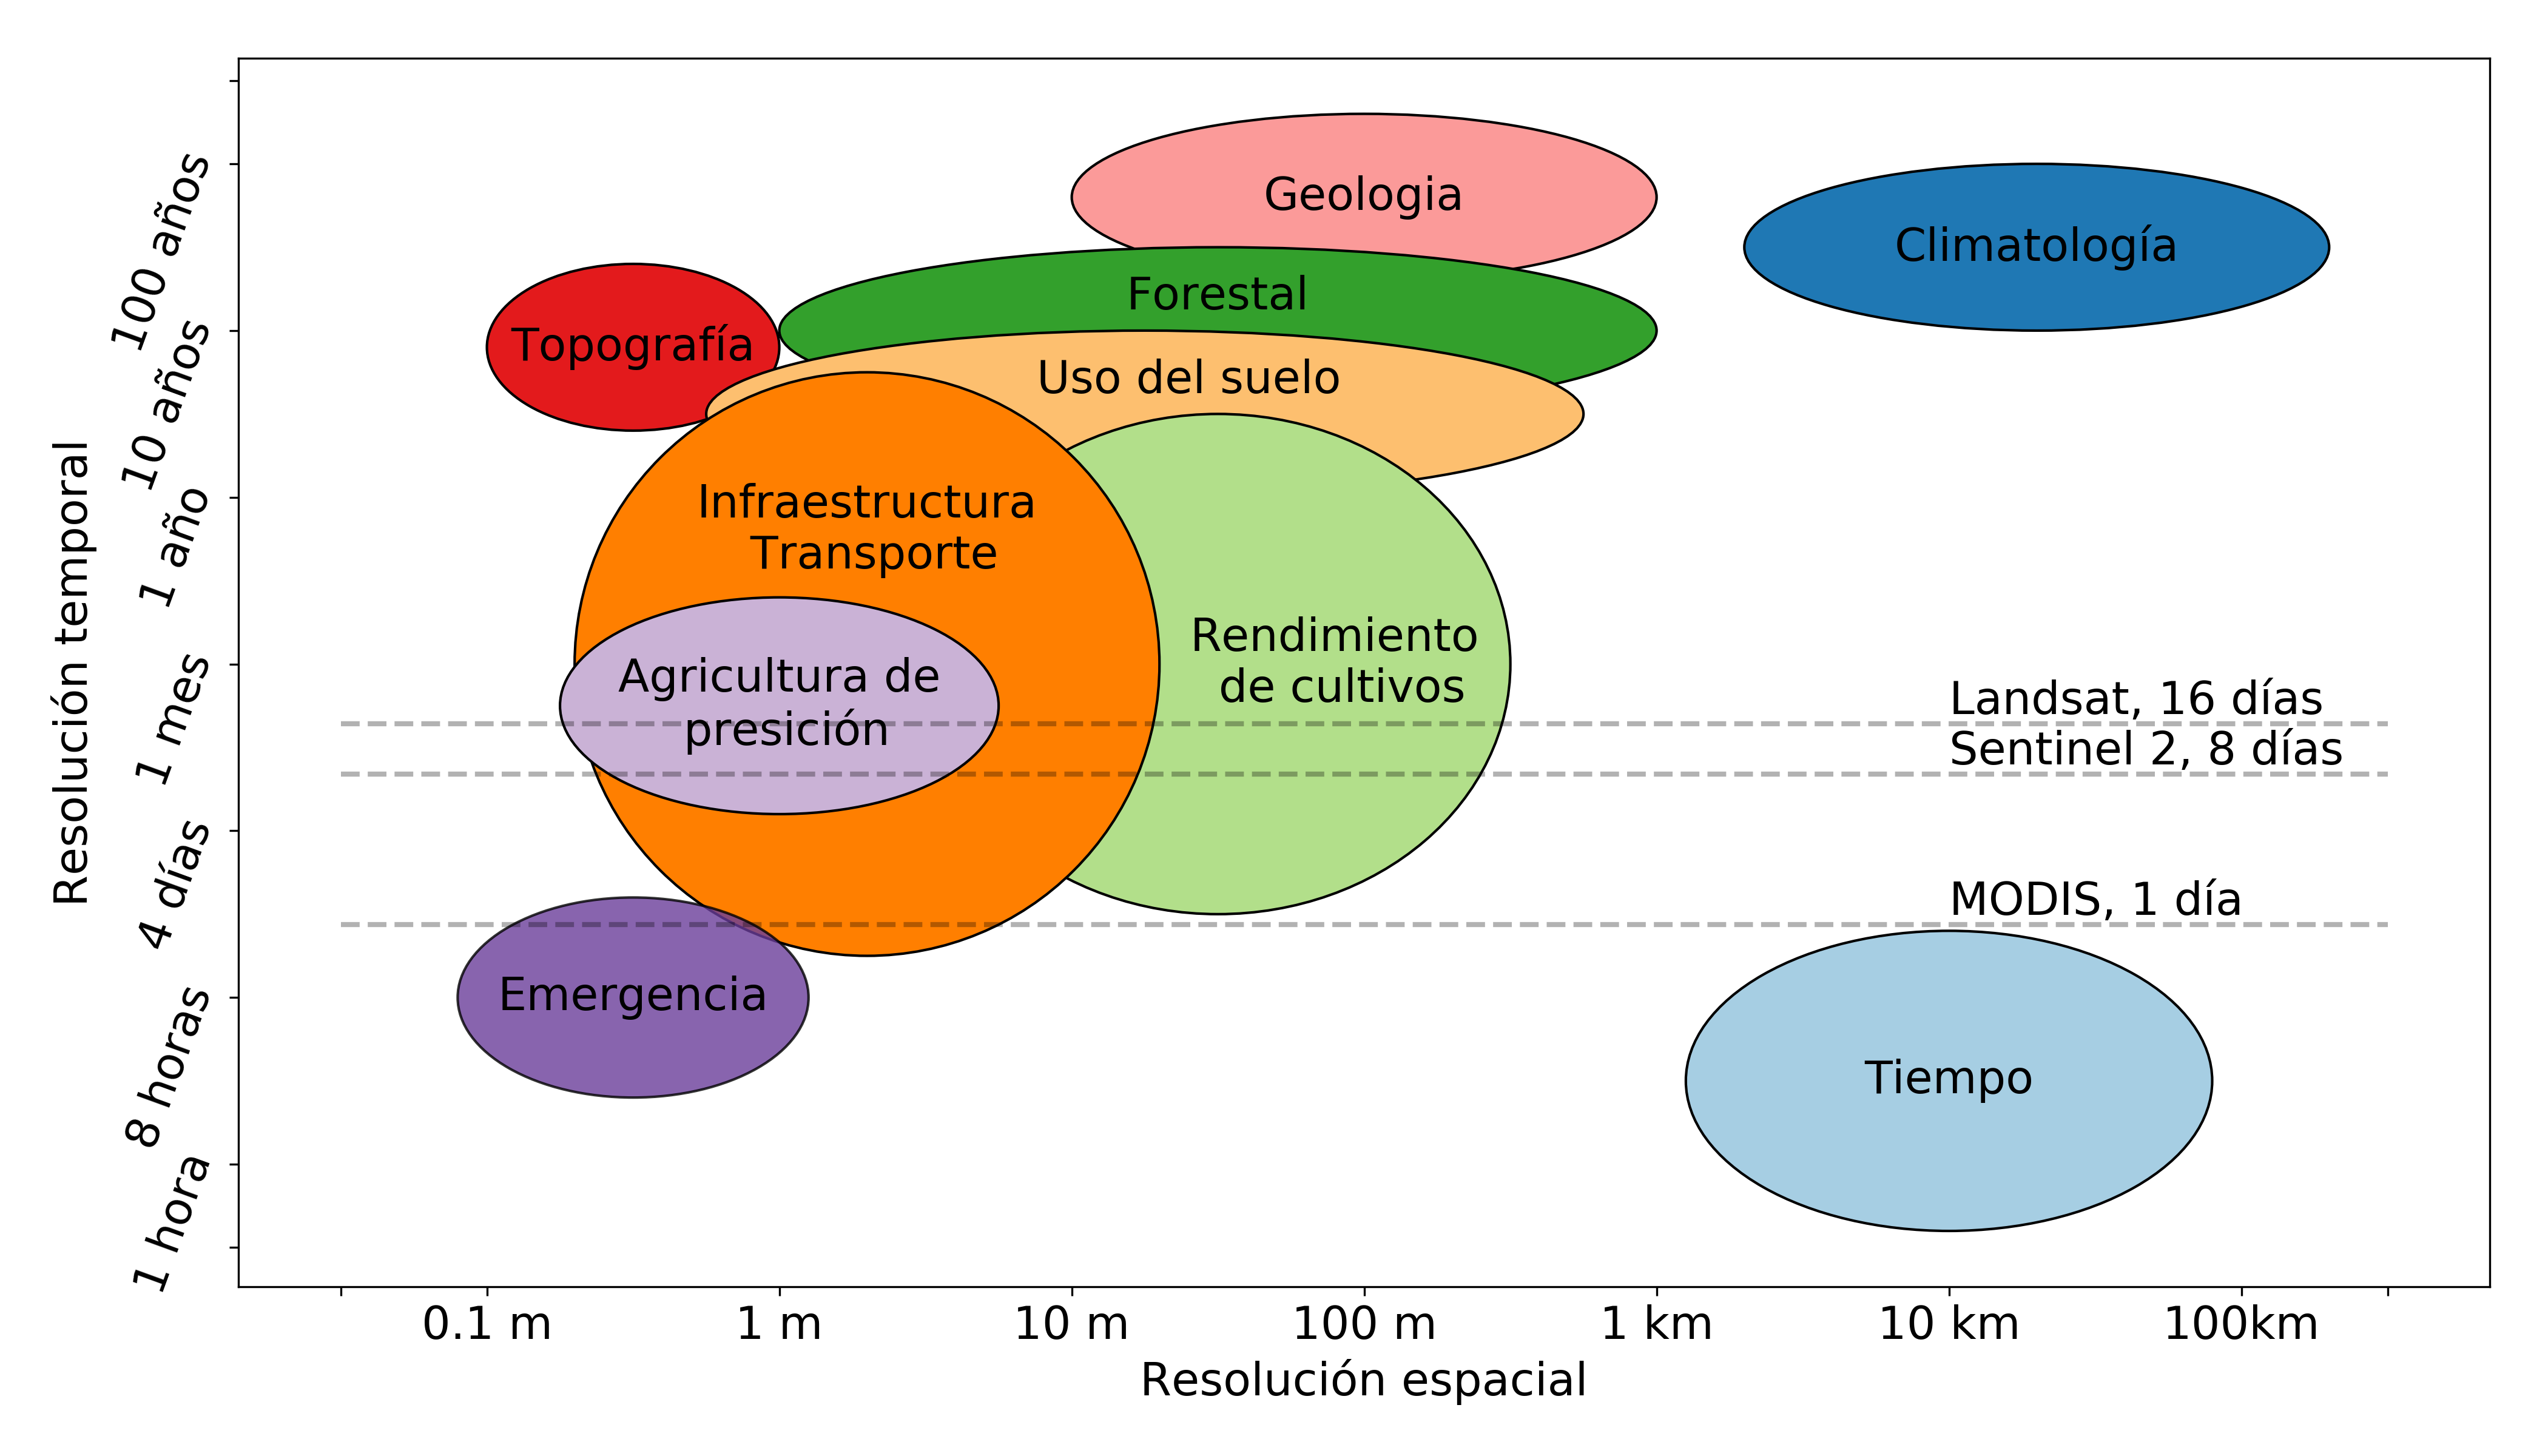
\includegraphics[width=0.85\textwidth]{fig:evst.png}
    \caption{}
    \label{fig:evst}
\end{figure}


Ambas resoluciones suelen estar relacionadas (Figura \ref{fig:evst}), de forma  tal que al aumentar una disminuye la otra. Por ejemplo: GOES, un satélite meteorológico, tiene alta revisita temporal (aproximadamente de 15 minutos), mientras que su resolución espacial es baja (4km). En el otro extremo, SPOT 7 tiene una alta resolución espacial, de hasta $1.5$m, pero con una revisita temporal del orden del mes.

Es importante destacar que no existen mejores o peores imágenes, sino que su elección dependerá del objeto de estudio.

\section{Imágenes satelitales}
Para seleccionar una imagen es necesario definir un area de interes (AOI), la herramienta "Draw rectangular"   %poner el icono o marcar en la figura.
En este caso dibuje un rectanglo que incluya la zona entre el Lago San Roque y Córdoba (Figura \ref{fig:aoi}) y seleccione el satélite Landsat 8 desde % poner el icono o mostrar en la imagen.
A continuación, en el margen derecho, aparecerán todas las escena disponibles.

\begin{figure}[h!]
    \centering
    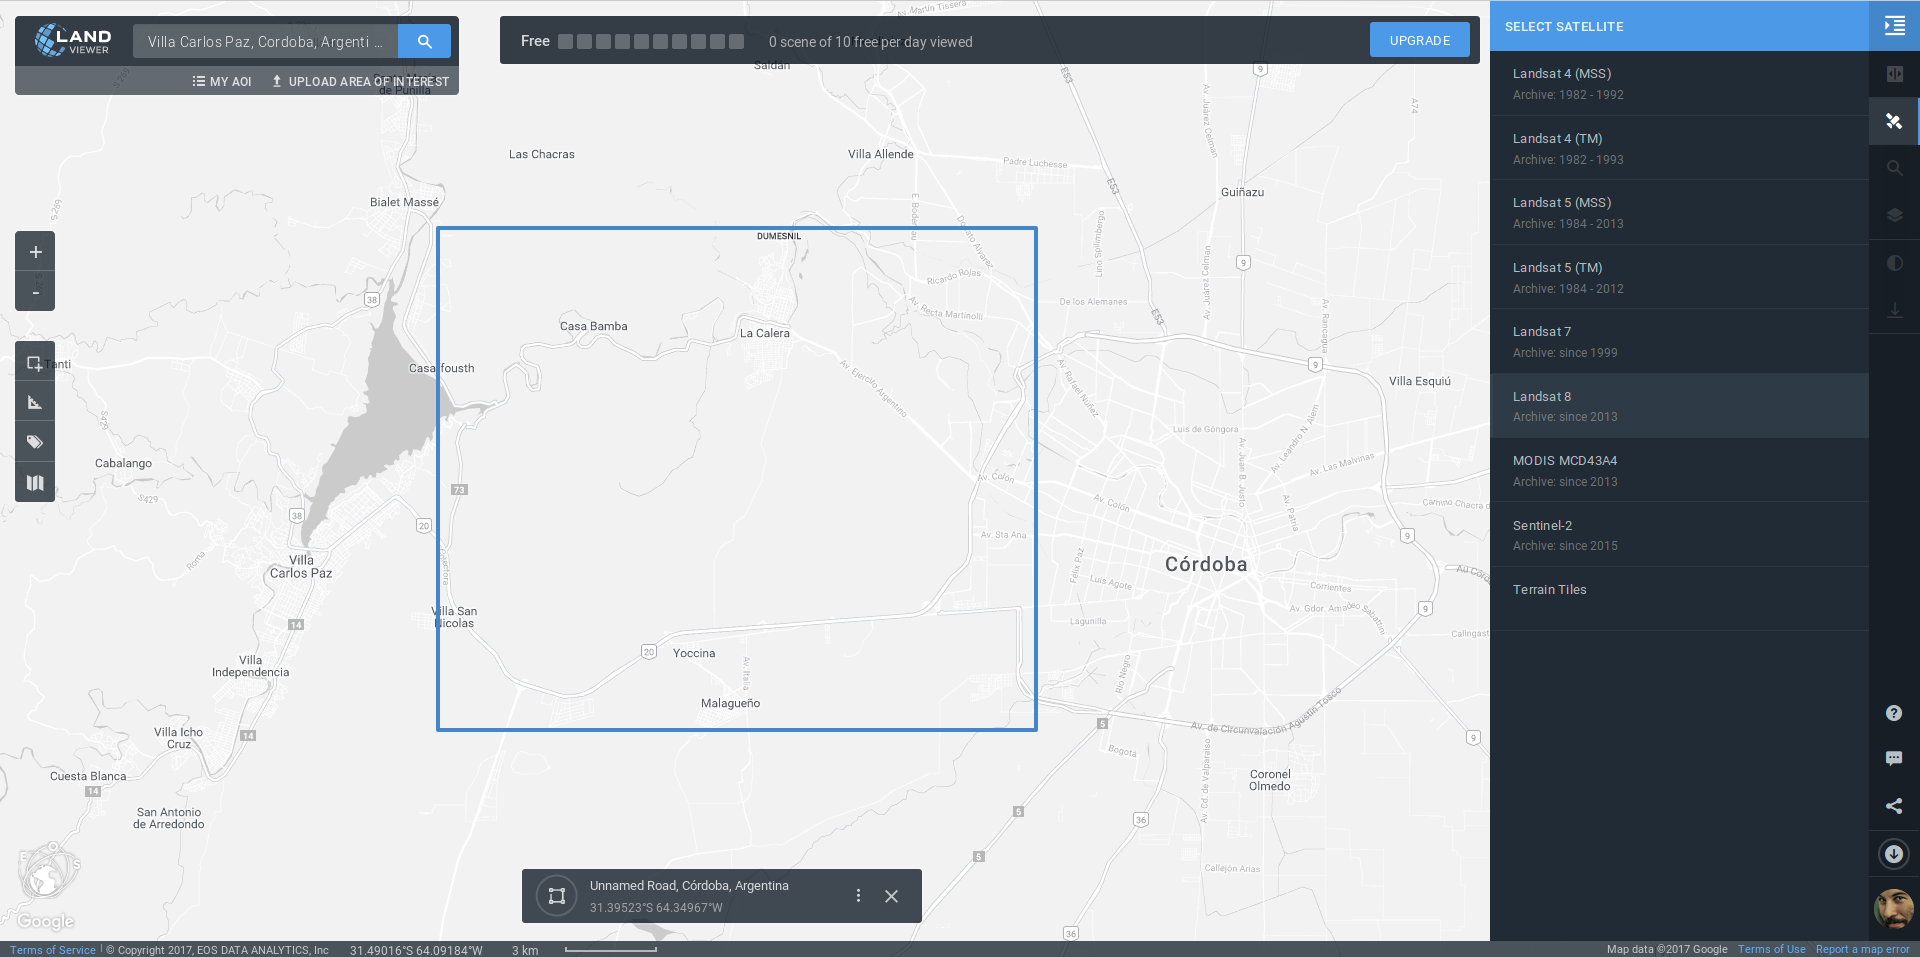
\includegraphics[width=0.85\textwidth]{fig:aoi.png}
    \caption{Gráfico de un área de interes (AOI) para seleccionar la zona en la que se seleccionaran las imagenes.}
    \label{fig:aoi}
\end{figure}

 Por defecto, Land Viewer muestra solo aquellas escenas que poseen una cobertura nubosa de hasta un 60\% y de los últimos 3 meses. Es posible cambiarlo haciendo click en la parte superior del Scene Search.  Modifique la cobertura nubosa al 100\%.
%yo pondria la captura con el grafiquito de nubes desplegado
\begin{center}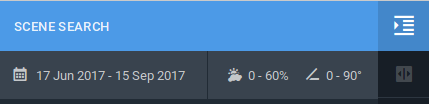
\includegraphics[scale=0.4]{in:nubes.png}\end{center}

Elija la imagen del 2 de Septiembre de 2017 (Figura \ref{fig:scene}) y se mostrará sobre el mapa. Puede moverse sobre ella y realizar mediciones.

\begin{figure}[h!]
\centering
\begin{minipage}{.425\linewidth}
  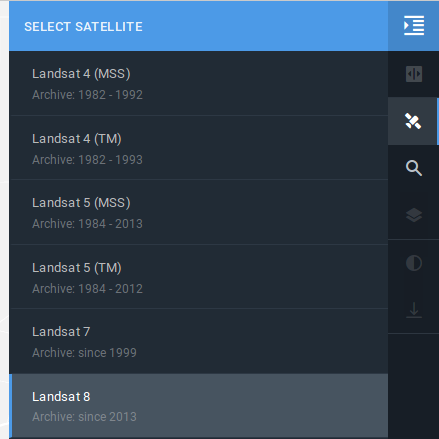
\includegraphics[width=\linewidth]{fig:sat.png}
\end{minipage}
\hspace{.05\linewidth}
\begin{minipage}{.425\linewidth}
  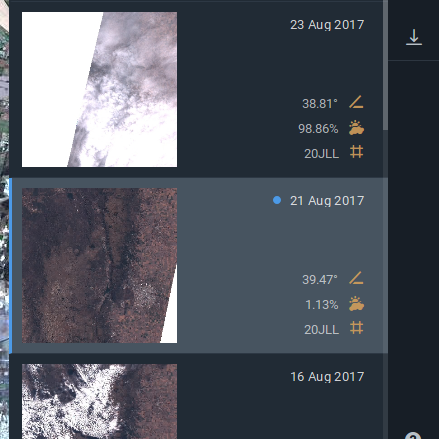
\includegraphics[width=\linewidth]{fig:imagen1.png}
\end{minipage}
\caption{Selección de satélite e imágenes en Land Viewer.}
\label{fig:scene}
\end{figure}

La imagen pertenece al sensor OLI del satelite Landsat 8, con una resolución espacial de $30m$, por lo tanto, solo podrá distinguir objetos de tamaño mayor como manzanas o parques, pero no más chicos.% ver
Vuelva a la lista de satélite y seleccione el producto MODIS MCD43A4, ahora encontrará una imagen por día. Seleccione la correspondiente al 27 de Agosto de 2017.

Observe que no es posible distinguir las manzanas de la ciudad de Córdoba como en el caso anterior. La imagen elegida pertenece al producto \emph{MCD43A4} generado a partir del sensor MODIS de los satélites AQUA y TERRA. Con una resolución espacial entre los 250m y los 1000m, según como mostremos la imagen.

\section{Comparación entre fechas}
Realice la comparación entre una imagen anterior y una porsterior al incendio, correspondientes a la misma época, en años consecutivos. Para ello, seleccione el satélite Sentinel 2 y elija la imagen del 21 de Agosto de 2017. Haga click en \emph{Comparison slider} 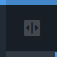
\includegraphics[scale=0.2]{in:LR.png} y seleccione la imagen del 23 de Agosto de 2016, modificando la fecha en el calendario.

Puede cambiar la posición de las imágenes a izquierda o la derecha con el botón L/R.

\begin{center}
\includegraphics[scale=0.4]{in:LorR.png}\end{center}

Desplace el slider a ambos lados y visualice la zona cercana al Lago San Roque (Figura \ref{fig:slider}).

\begin{figure}[h!]
    \centering
    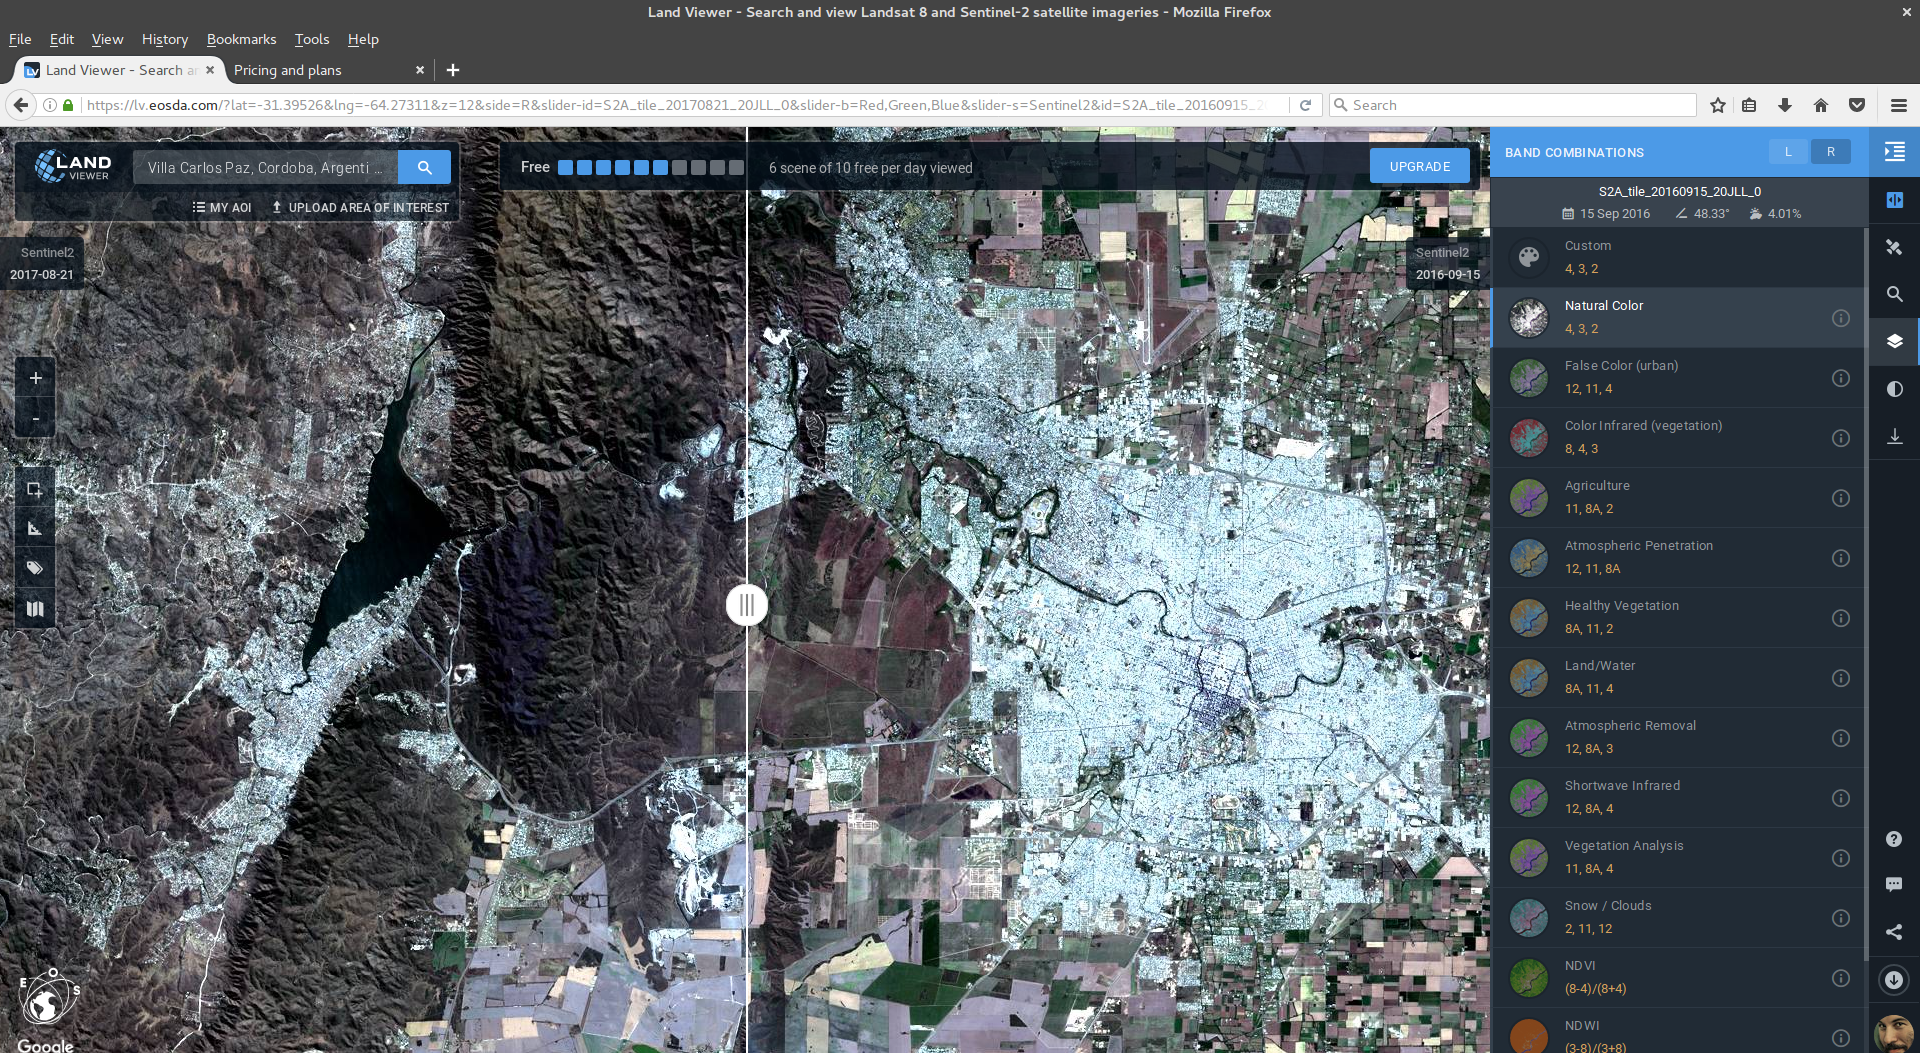
\includegraphics[width=0.85\textwidth]{fig:slider.png}
    \caption{Dos imágenes en pantalla, separadas por el slider que permite cambiar entre las dos zonas.}
    \label{fig:slider}
\end{figure}

\section{Actividades}
\begin{que}
    ¿Cada cuantos días hay una nueva imagen Landsat 8?
\end{que}
\begin{que}
    ¿Cada cuantos días hay una nueva imagen MODIS?
\end{que}
\begin{que}
    ¿Es posible distinguir las manzanas de la Ciudad de Córdoba en la imagen Landsat 8?
\end{que}
\begin{que}
    ¿Hay incendios en la zona durante el año 2016?
\end{que}
\begin{que}
    ¿Qué superficie tiene el área incendiada dentro de la imagen?
\end{que}

\chapter{Combinaciones espectrales}

Hasta ahora ha trabajado con imágenes cuya combinación de colores resulta intuitiva, pero no permite distinguir claramente las zonas incendeadas. Para mejorar esta situación se utilizaran zonas del espectro electromagnetico que normalmente no pueden ser distinguidas por el ojo humano, pero sí por el sensor.
Los satélite miden la cantida de luz que proviene de la superficie terrestre. Las distintas coberturas como vegetación, agua y suelo sin cobertura vegetal tienen comportamientos característico dentro del espectro, las cuales pueden ser utilizados para extraer información sobre ellos (Figura \ref{fig:spec}).



\begin{figure}[h!]
    \centering
    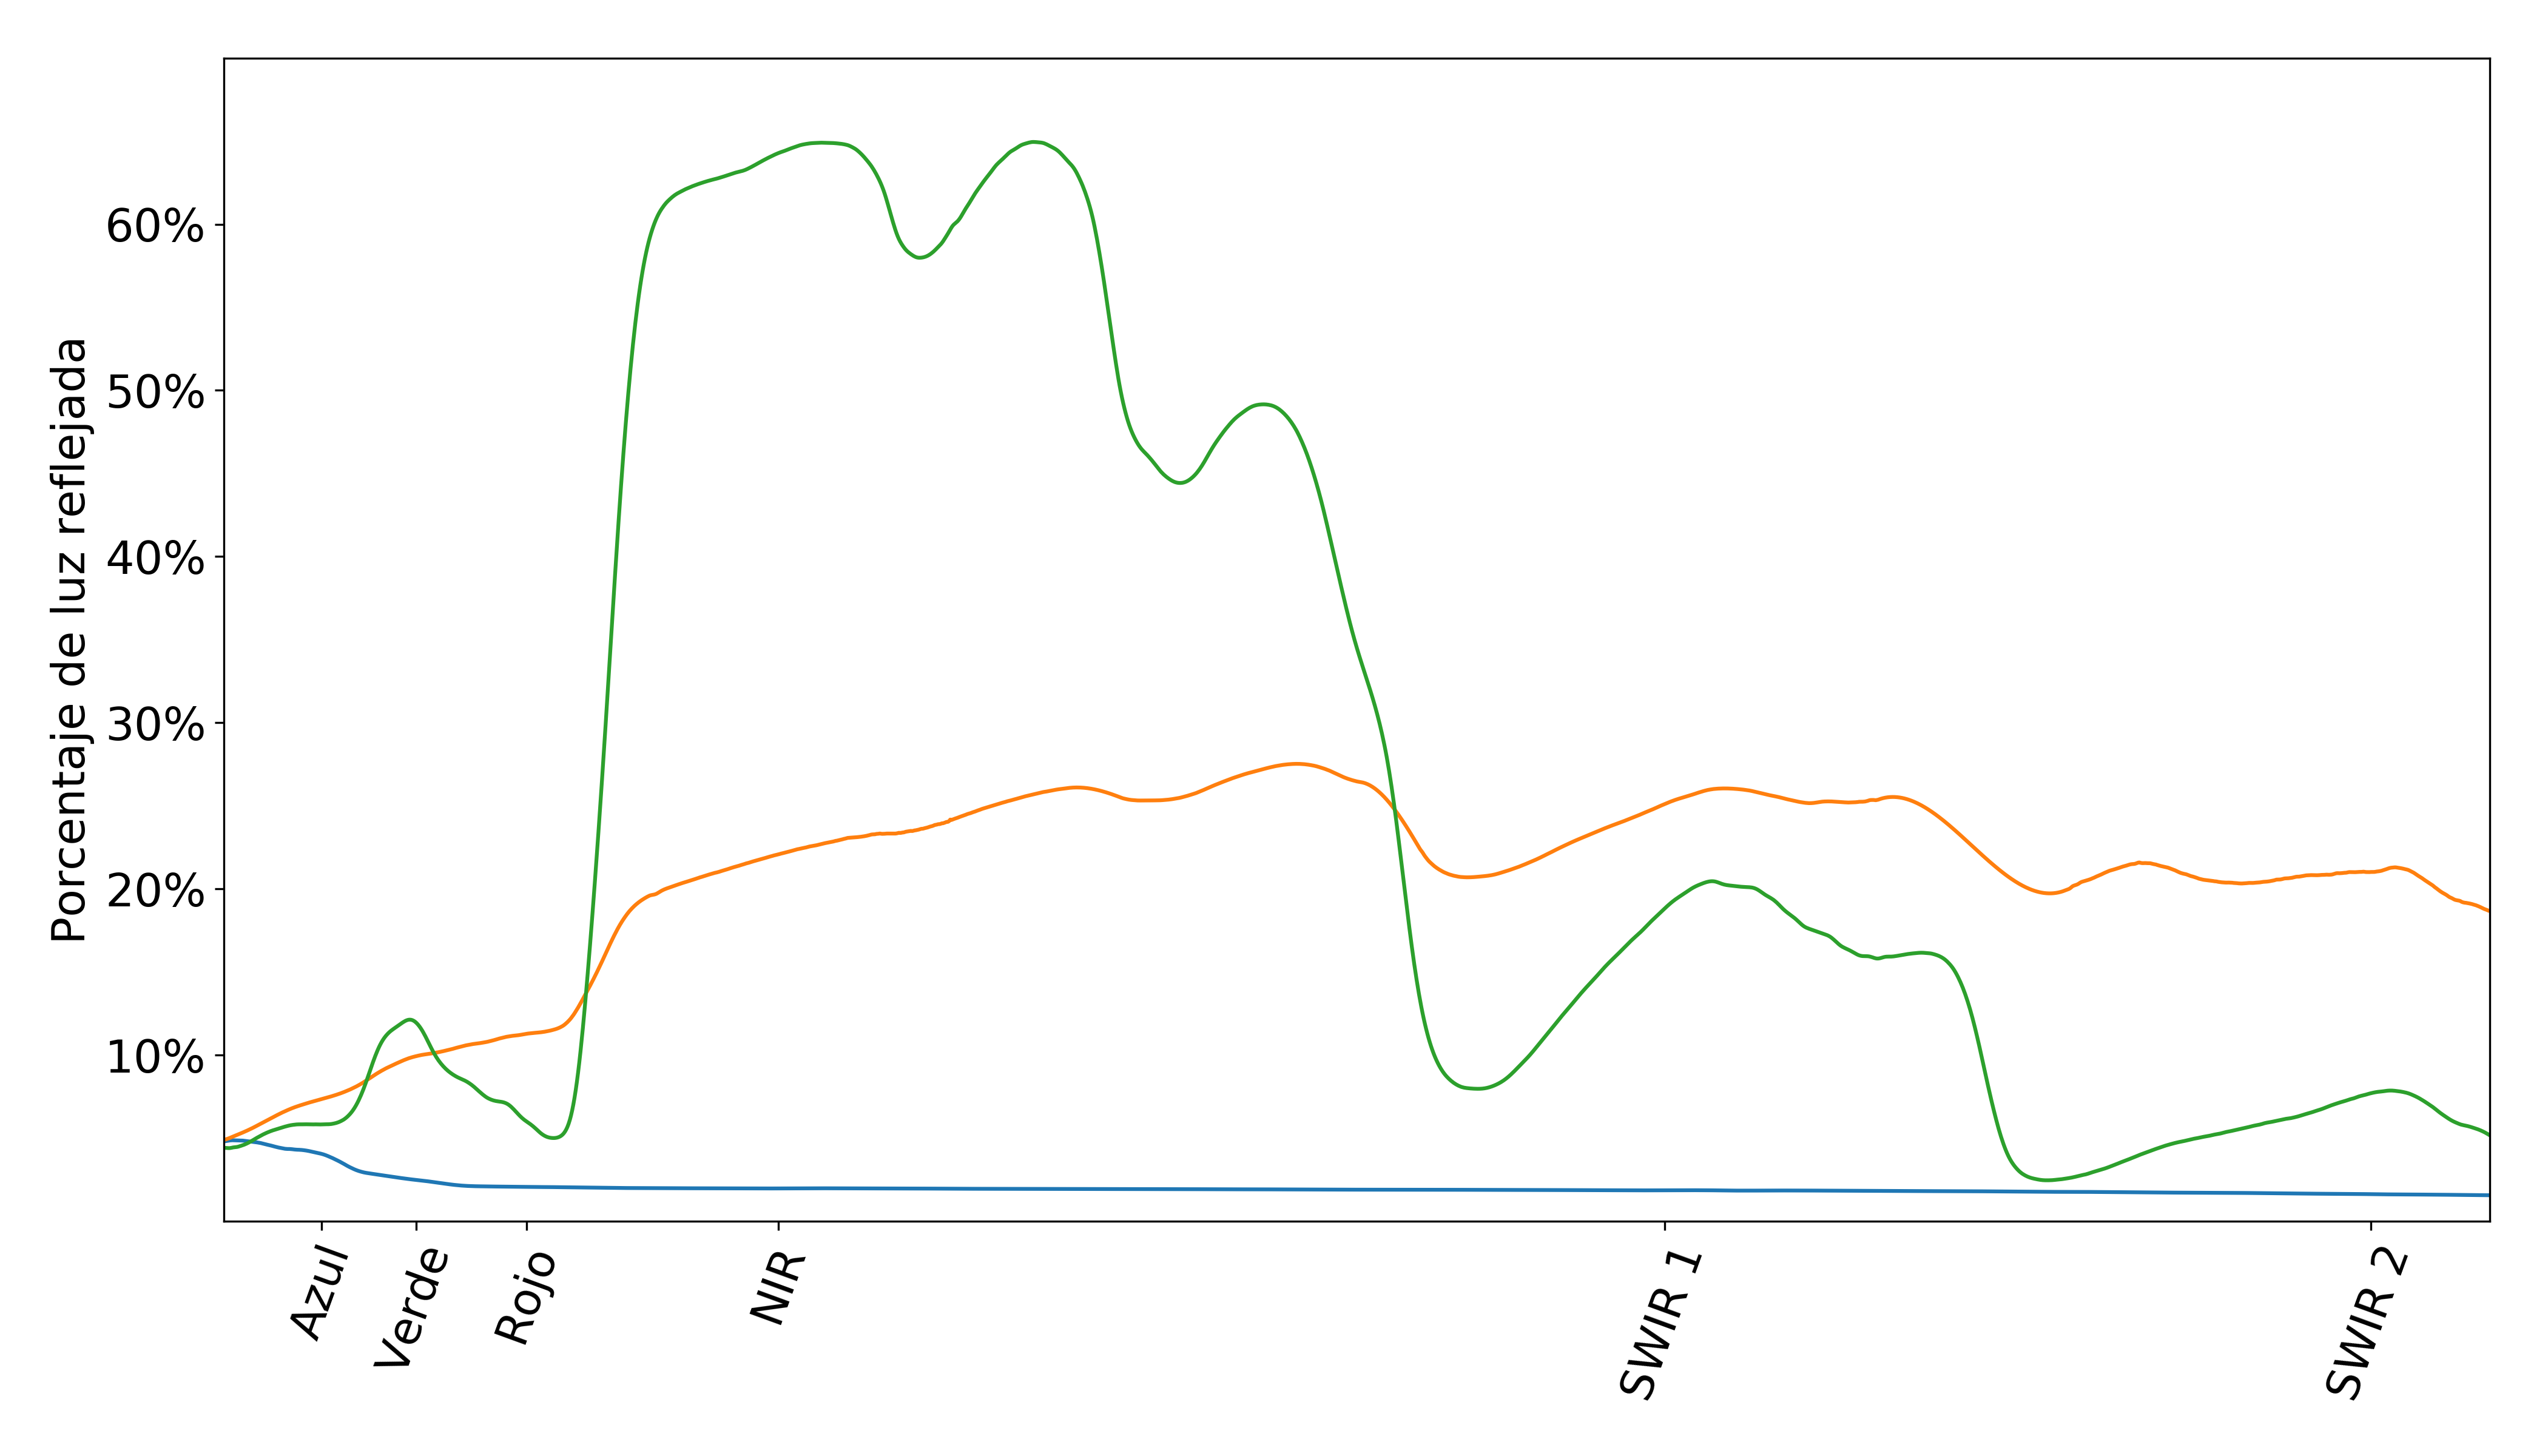
\includegraphics[width=0.85\textwidth]{fig:spec.png}
    \caption{Firmas espectrales para el agua, suelo y vegetación.}
    \label{fig:spec}
\end{figure}


\section{Combinaciones RGB}

Las combinaciones RGB permiten mostrar en color azul, verde y rojo la información de cada longitud de onda.

En Land Viewer, puede modificarlo haciendo click en BAND COMBINATIONS (Figura \ref{fig:bandas}).

\begin{figure}[h!]
    \centering
    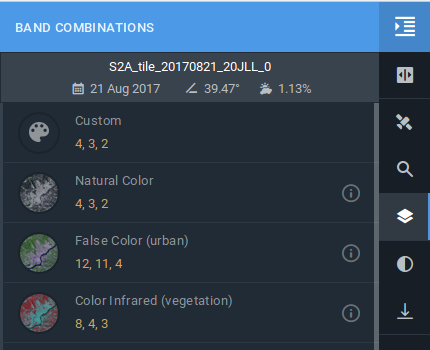
\includegraphics[width=0.4\textwidth]{fig:bandas.png}
    \caption{Ventana de combinaciones de bandas. Es posible elegir una disponible o configurar una nueva.}
    \label{fig:bandas}
\end{figure}

Las combinaciones espectrales permiten mostrar distinta información:

\begin{itemize}
    \item Color real (\emph{Natural color - rojo,verde,azul}): Muestra la imagen de forma similar a como la verían nuestros ojos. La vegetación se ve verde, los suelos en distintos tonos de marrón, las ciudades en blanco y los cuerpos de agua se observan en colores oscuros.
    \begin{center}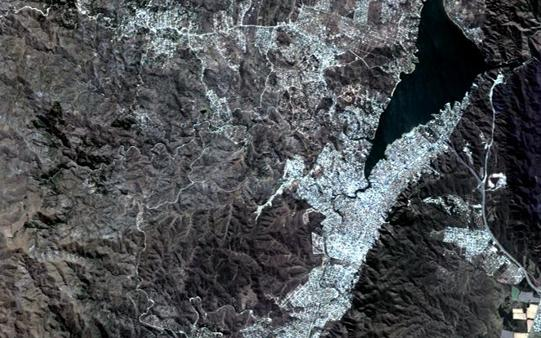
\includegraphics[scale=0.3]{4-3-2.jpeg}\end{center}
    \item Falso color (\emph{False color (urban) - SWIR2,SWIR1,Rojo}): Proporciona una interpretación similar a la observada por el ojo humano, sin tener en cuenta la incidencia de la atmosfera. La vegetación se visualiza en verde, las zonas urbanas en blanco y ciam, los suelos en una variedad de colores y las zonas con agua se notan en azul o negro.
    \begin{center}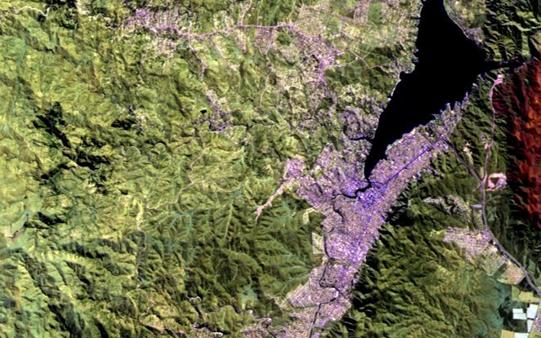
\includegraphics[scale=0.3]{12-11-4.jpeg}\end{center}
    \item Infrarrojo color (\emph{Color infrared (vegetation) - NIR, Rojo, Verde}): La combinación de color hsbitual para separar vegetación de otras coberturas. Auí la vegetación suele verse en color rojo brillante, las ciudades y suelos sin cobertura en tonos de cian y las zonas con agua se ven en negro.
    \begin{center}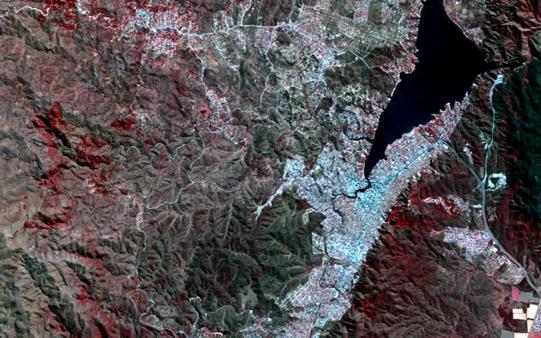
\includegraphics[scale=0.3]{8-4-3.jpeg}\end{center}
    \item Falso color (\emph{Land/water - NIR, SWIR1, Rojo}): Combinación de bandas útil para caracteriza la vegetacion y separarla de la cobertura agua. La vegetación se verá en tonos de naranja, dependiendo de su contenido de humedad, las zonas con agua en azul y las ciudades y el suelo desnudo en  color blanco o verde.
    \begin{center}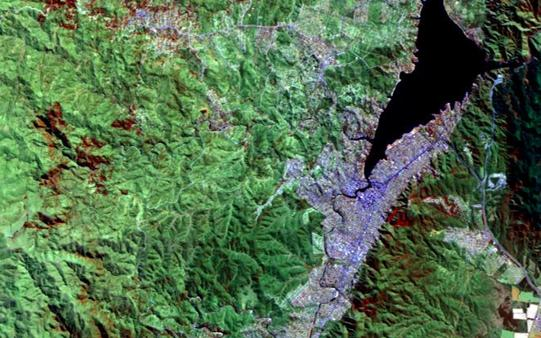
\includegraphics[scale=0.3]{8-11-4.jpeg}\end{center}
\end{itemize}

En nuestro caso particular, la combinación espectral que mejor separa las zonas incenciadas de las no incendiadas es la \emph{Short wave infrared}, donde se muestra en rojo las zonas que se incendiaron recientemente y en verde las zonas con vegetación. Seleccione la combinación en Land Viewer y compare ambas imágenes. (Figura \ref{fig:incendio}).

\begin{figure}[h!]
    \centering
    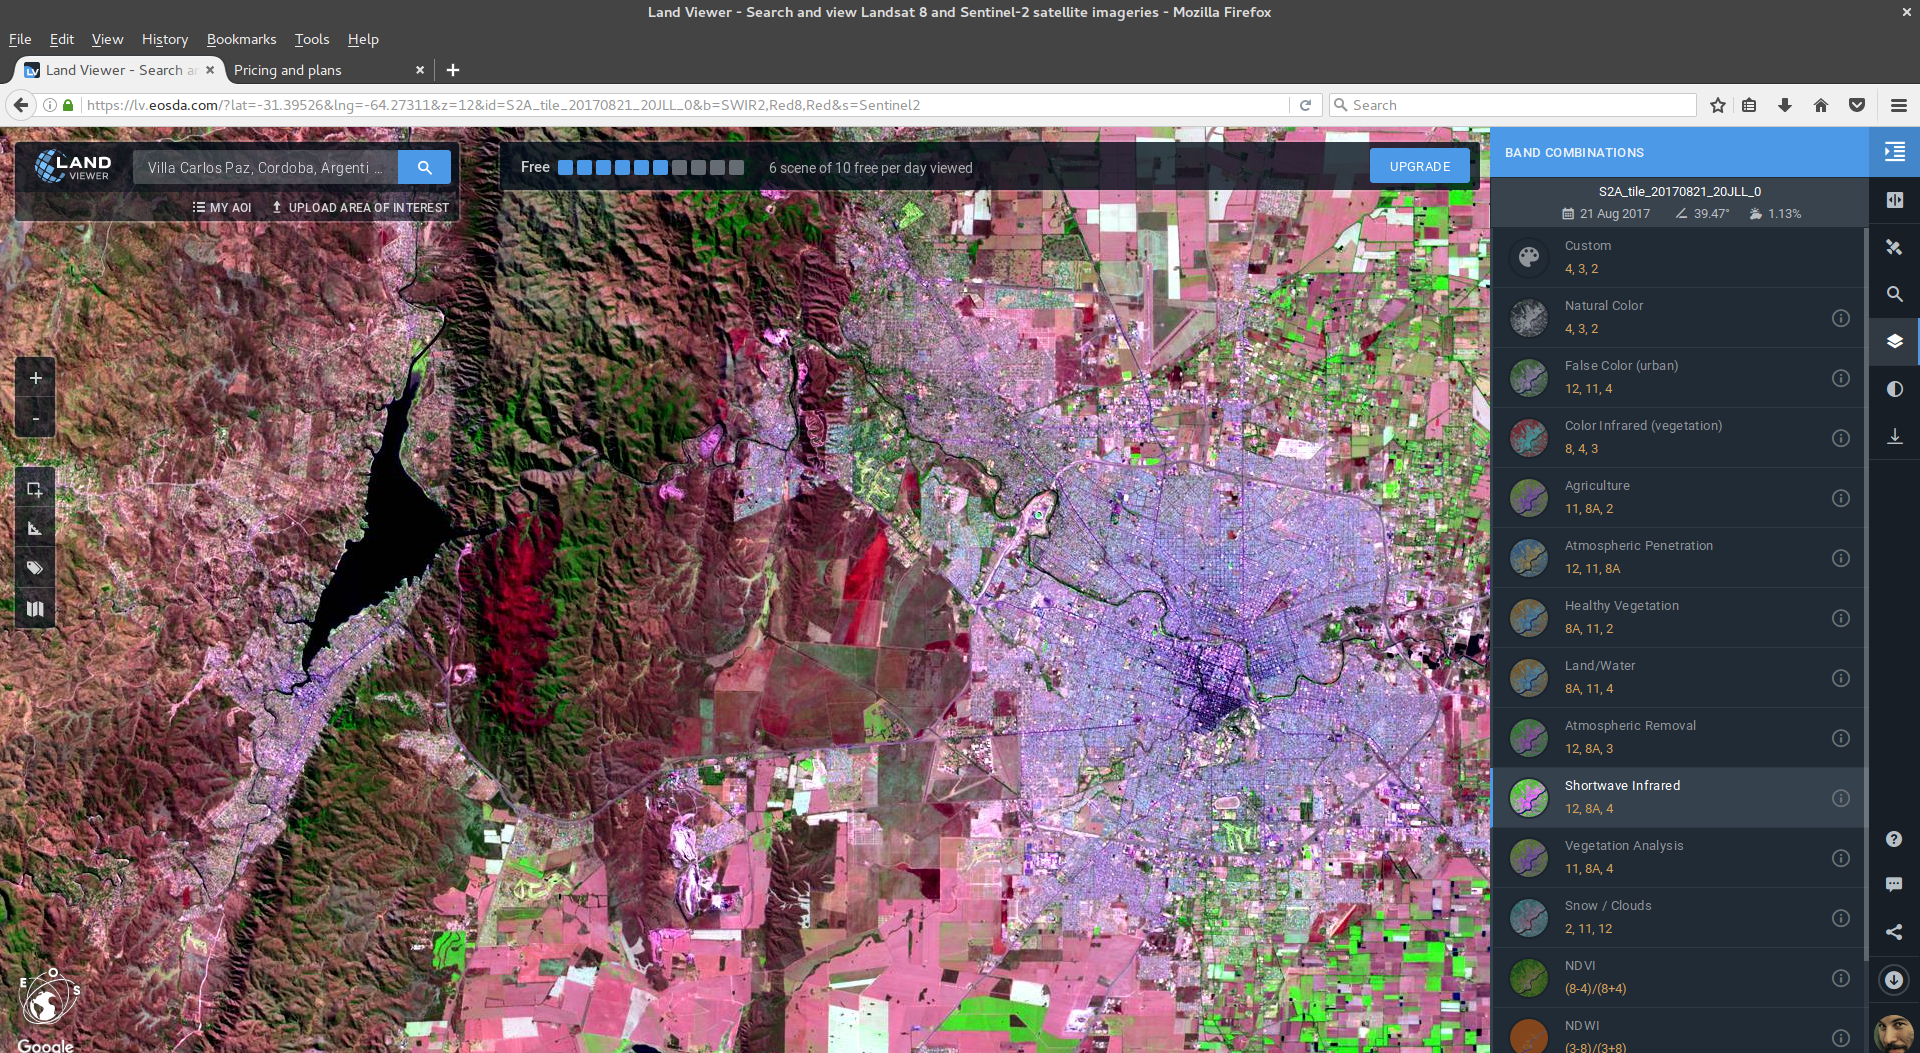
\includegraphics[width=0.85\textwidth]{fig:incendio.png}
    \caption{Imagen en combinación espectral \emph{Short wave infrared}. La vegetación se observa en colores verde brillante, el incendio en rojo, el agua en negro y la ciudad en violeta.}
    \label{fig:incendio}
\end{figure}

Puede descargar la imagen generada haciendo click en ESCENE DOWNLOAD, elija la opción  \emph{Crop by extent} y luego haga click en Download.

\section{Actividades}

\begin{que}
    ¿Cuál es la superficie incendiada al oeste del Lago San Roque?
\end{que}

\begin{que}
    ¿En qué color se visualiza la zona incendiada en cada una de las combinaciones de bandas descriptas arriba?
\end{que}

\begin{que}
    ¿Qué combinación espectral le permite distinguir más detalles en el Lago San Roque?
\end{que}

\begin{que}
    ¿Qué combinación espectral le permite distinguir vegetación dentro de la ciudad de Córdoba?
\end{que}

\begin{que}
    ¿Cuanto creció la superficie incendiada entre el 21 de Agosto y el 17 de septiembre de 2017 al este de Villa Carlos Paz?
\end{que}

\begin{que}
    Descargue un mapa de la zona donde se vea la superficie incendiada al 21 de Agosto de 2017 en la cercanía de Villa Carlos Paz.
\end{que}

\chapter{Cierre}

En este taller se mostró como utilizar las herramientas de LandView junto con algunos conceptos basicos de teledetección, para interpretar imágenes.

Aprendimos que hay 3 características fundamentales de un conjunto satélite/sensor para el uso de productos geoespaciales

\begin{itemize}
    \item Resolución espacial: capacidad de distinguir un objetos en el terreno.
    \item Resolución temporal: cada cuanto tiempo se tiene una imagen de la misma zona.
    \item Resolución espectral: csntidad de zonas del espectro que se pueden distinguir.
\end{itemize}

Esta es una primera aproximación al trabajo en teledetección, donde la interpretación visual se combina con el procesamiento digital para extraer información sobre la superficie terrestre. 


\end{document}
